\chapterauthor{Author Name1}{Affiliation text1}
\chapterauthor{Author Name2}{Affiliation text2}
\chapterauthor{Author Name3}{Affiliation text3}
\chapterauthor{Author Name4}{Affiliation text4}

\chapter{Multi objective evolutionary algorithms applied to Protein Structure Prediction Problem}

\section{Introduction} \label{sec:intro}

%Objetivos

%Contribuições

\section{Protein folding} \label{sec:psp}


We will briefly recall some of the main biological concepts related to the protein folding problem that are relevant to our discussion.


Proteins are macromolecules made out of  twenty different amino acids, also referred to as residues. An amino acid has a peptide backbone and a distinctive side chain group. The peptide bond is defined by an amino group and a carboxyl group connected to an alpha carbon to which a hydrogen and side chain group are attached.


Amino acids are combined to form sequences which are considered the primary structure of the peptides or proteins. The secondary structure is the locally ordered structure brought about via hydrogen bounding mainly within the peptide backbone. The most common secondary structure  elements in proteins are the alpha helix and the beta sheet. The tertiary structure is the global folding of a single polypeptide chain.


Under specific conditions, the protein sequence folds into a unique native 3-d structure. Each possible protein fold has associated energy. The \emph{thermodynamic hypothesis} states that the native structure of a protein is the one for which the free energy achieves the global minimum. Based on this hypothesis, many methods that search for the protein native structure define an approximation of the protein energy and use optimization algorithms that look for the protein fold that minimizes this energy. These approaches mainly differ in the type of energy approximation employed and in the characteristics of the protein modeling.


The achievement of the protein native structure is the result of the so-called protein folding process. The laws that govern protein folding are unknown. Therefore a number of ideas have emerged that try to answer this question: how do amino acid sequences specify proteins 3-d structure?


There are two main approaches to protein folding, commonly referred as the ``classical'' and ``new'' views. The ``classical'' view considers folding as a defined sequence of states leading from the unfolded to the native state.  This sequence is called the pathway \cite{pande:1998}. In the  ``new'' view approach,   folding is seen as the progressive organization of an ensemble of partially folded structures  through which the protein passes on its way to the folded structure \cite{onuchic:2004}. This approach emphasizes the idea of each state being an ensemble of rapidly interconverting conformations. One of the main differences between both approaches is that the ``new'' view allows for a more heterogeneous transition state than the ``classical'' view, which concentrates on a single, well-defined folding pathway \cite{baker:2000}.


Figure~\ref{fig:protviews}  shows one schematic representation of the ``classical'' (left) and  ``new'' (right) views of protein folding. In the figure, each possible protein configuration is represented as a circle, and arrows represent possible transitions between configurations. In both approaches, the native state (filled circle) is achieved when the energy is minimized.


\begin{figure}[htb!]
	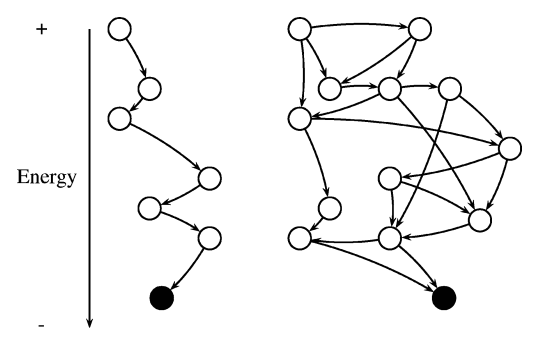
\includegraphics[scale=.6]{figures/protviews.png}
	\label{fig:protviews}
	\caption{Schematic representation of the “classical” (left) and “new” (right)
		views of protein folding.}
\end{figure}


%Citar outros operadores (referenciar trabalhos)


%Mencionar abordagens multi-objetivo (referenciar trabalhos)


\section{Multi-objective Optimization} \label{sec:optimization}


Evolutionary Algorithm (EA) is a optimization and search technique, highly parallel, inspired by the Darwinian principle of natural selection and genetic reproduction. The nature principles that inspire the EAs are simple. According to the theory of C, Darwin, the principle of natural selection favors individuals with high fitness, therefore, with high probability of reproduction. Individuals with more descendants have more chance to perpetuate their genetic code in future generations. The genetic codes is what gives the identity of each individual and are represented in the chromosomes. These principles are used in the construction of computational algorithms, that searches for better solutions given a specific problem by the evolution of a population of solutions coded in artificial chromosomes -- data structures used to represent a feasible solution for a given problem in the algorithm execution \cite{pacheco1999algoritmos}.


Real world problems commonly have multiple objectives to minimized/maximized and are present in most knowledge areas. To optimize multi objective problems, are considered two or more objectives witch usually are conflicting. To these problems is impossible to find one unique solution. A set of solutions is reached evaluating the Pareto dominance relation \cite{pareto} between the solutions. The main objective is to find the solutions that are non-dominated by any other. A solution dominates other, if and only if, it was better in at least one of the objectives, without being worst in any of the objectives. The set of non-dominated solutions constitutes the Pareto Front. Finding the the real Pareto Front is a NP-hard problem \cite{fonseca2005tutorial}, this way, the objective is to find a good approximation of this front.


Multi-Objective Evolutionary Algorithms (MOEAS) are extensions of EAs to multi objective problems that applies the concepts of Pareto dominance to create different strategies to evolve and diversify the solutions. In this work were used two MOEAs: NSGAII \cite{deb2002fast} and IBEA \cite{zitzler2004indicator}.


\subsection{Non-dominated sorting Genetic Algorithm II}


The main characteristic of this algorithm is a strong elitism mechanism, classifying at each generation every solution in different fronts according with the non-dominance relation (line 15 of Algorithm \ref{alg:nsgaII}). After the classification, solutions from the first front, are non-dominated by any other solution. Solutions from the second front are dominated only by the solutions of the first front, and so on. For solutions of the same front, the algorithm uses a Crowding Distance operator to calculate how distant are the neighbors of a given solution (line 19 of Algorithm \ref{alg:nsgaII}). Solutions with high values of Crowding Distance have priority, because they will contribute more to the population's diversity. The binary tournament selects solutions from the small front with the higher values of Crowding Distance. A new population is generated using the crossover and mutation operators (line 25 of Algorithm \ref{alg:nsgaII}).


\begin{algorithm}[h]
	\begin{algorithmic}[1]
		\State{$N \gets$ Population Size}
		\State{$T \gets$ Max evaluations}
		\State{$P_0 \gets CreatePopulation(N);$}
		\State{$CalculateFitness(P_0);$}
		\State{$FastNonDominatedSort(P_0);$}
		\State{$Q_0 \gets 0$}
		\While{$Q_0 < N$}
			\State{$Parents \gets BinaryTournament(P_0);$}
			\State{$Children \gets CrossoverMutation(Parents);$}
			\State{$Q_0 \gets Children$}
		\EndWhile
		\State{$CalculateFitness(Q_0);$}
		\State{$t \gets 0$}
		\While{$t < T$}
			\State{$R_t \gets P_t \cup Q_t;$}
			\State{$Fronts \gets FastNonDominatedSort(R_t);$}
			\State{$P_{t+1} \gets 0$}
			\State{$i \gets 0$}
			\While{$P_{t+1} + Front_i  < N$}
				\State{$CrowdingDistanceAssignment(Front_i);$}
				\State{$P_{t+1} \gets P_{t+1} \cup Front_i$}
				\State{$i \gets i + 1$}
			\EndWhile
			\State{$CrowdingDistanceSort(Front_i);$}
			\State{$P_{t+1} \gets P_{t+1} \cup Front_i[1:(N -P_{t+1})]$}
			
			\State{$Parents \gets BinaryTournament(P_{t+1});$}
			\State{$Q_{t+1} \gets CrossoverMutation(Parents);$}
			\State{$t \gets t +1$}
		\EndWhile
		\State{\Return{$P \gets$ Set of non-dominated solutions.}}
	\end{algorithmic}
	\caption{NSGAII}
	\label{alg:nsgaII}
\end{algorithm}


\subsection{IBEA (Indicator-Based Evolutionary Algorithm)}


In the multi-objective optimization context, optimizing consists in find a front with a good approximation to the true Pareto front. However, there is no general definition about what is the true Pareto front. This way, indicators have been used to evaluate the quality of a approximation front. The \textit{hypervolume} is a example of indicator to the evaluation and comparison of fronts.


The IBEA is an algorithm that considers the optimization by the use of quality indicators. The indicator is the way used to evaluate the non-dominated set of solutions \cite{figueiredo2013algoritmo}. To use the IBEA it is necessary define which indicator will be used to associate each ordered pair of solutions to a scalar value. One of the most used indicators is the \textit{hypervolume} due to its capacity of evaluate the convergence and diversity at the same time of the search process \cite{ishibuchi2008evolutionary}.


\begin{equation} \label{eq:ibea_fitness}
F(x_i) = \sum_{x_j \in (P-x_i)} {-e^\frac{-I_{Hy}(x_j,x_i)}{k}}
\end{equation}


For the IBEA fitness calculation (Equation \ref{eq:ibea_fitness}), $k$ is a parameter commonly used with a value of 0.05. The value for $F(x_i)$ corresponds to a quality loss measure of the approximation to the Pareto front if the solution $x_i$ was removed of the population \cite{figueiredo2013algoritmo}, based on the value of the quality indicator $I_{Hy}$, in this case, the \textit{hypervolume}. Based on the fitness calculation described above, the basic IBEA algorithm consists in iteratively do the selection (line 10 of Algorithm \ref{alg:ibea}), crossover, mutation (line 11 of Algorithm \ref{alg:ibea}) and environment selection, removing the worst individual from the population and updating the values of fitness of the remaining individuals (lines 4 to 8 of Algorithm \ref{alg:ibea}).


\begin{algorithm}[h]
	\begin{algorithmic}[1]
	\State{$N \gets$ Population Size}
	\State{$T \gets$ Max Evaluations}
	\State{$k \gets$ Scale factor of Fitness}
	
	\State{$P \gets$ CreatePopulation($N$);}
	\State{$m \gets 0$}
	\State{CalculateFitness($P$);}
	
	\While{$m \ge T$ or other stop criterion is reached}
		
		\State{$\overline P \gets$ BinaryTournament($P$);}
		\State{$P \gets$ CrossoverMutation($\overline P$);}
		\State{$m \gets m+1$}
		
		\While{Size($P$) $> N$}
			\State{$x^* \gets$ WorstIndividualByFitness();}
			\State{RemoveFromPopulation($x^*$, $P$);}
			\State{CalculateFitness($P$);}
		\EndWhile
	
	\EndWhile
		\State{\Return{$P \gets$ Set of non-dominated solutions}}
	
	\end{algorithmic}
	\caption{IBEA}
	\label{alg:ibea}
\end{algorithm}


\footnotetext[1]{\textit{Hypervolume}: Proposed quality indicators used in the study of \cite{zitzler1998multiobjective}, denoted as the "size of the covered search space". This indicator has two important advantages in relation to others \cite{zitzler2007hypervolume}: 1 - Sensitive to any kind of improvement in the approximation set in relation to other set. 2 - As result of 1, the indicator guarantee that for any approximation set $A$ that has high values of hypervolume, also has all the solutions of the true Pareto front.}


\section{Proposed method}
\label{sec:proposedMethod}


Two multi-objective approaches were designed in this paper and will be presented in this section.  The first approach consisted on applying two well-known state of art multi-objective algorithms (IBEA and NSGAII) to the PSP using the HP-2D model.  The genetic operators used by IBEA and NSGAII algorithms, in this approach, were only the single point crossover in the case of crossover and bit flip mutation for mutation operator.  It was decided to use only single point crossover and bit flip mutation, in this approach, because this combination of operators presented better results in previous experiments within the PSP problem with HP-2D model.

In the case of the second approach the IBEA and NSGAII algorithms were modified in order to improve their results when compared with the first approach. The modifications will be described next:

\begin{itemize}
	\item \textbf{Backtrack Initialization}: Traditionally the initial population of solutions are generated randomly in MOEAs. This have a great potential of generating a large number of invalid solutions for the PSP problem. Solutions that are not self-avoiding walk (SAW) are said to contain collisions. If the initial population is fully generated randomly the evolutionary algorithms will spend time processing invalid solutions until getting good results. In order to subdue this problem a backtrack strategy should be applied. In this approach 20 percent of the initial population were generated using the backtrack strategy.
	\item \textbf{Design of specialized genetic operators}:  As mentioned in section X, the use of traditional operators usually does not guide the search to prominent regions of the search space of the HP-2D model. In order to supplement the MOEAs, a pool of operators were designed based on the literature and are presented on table X.  For every mating the crossover and mutation operators are selected randomly from the pool of operators. Also the crossover and mutation operators are always applied differently from the first approach which uses a probability of occurence. 
\end{itemize}

For both approaches the same objectives were used and will be explained  at next:

\begin{itemize}
	\item \textbf{Energy value}: This is the main objective and consist in the energy of given protein conformation.  The goal is to minimize the energy value and it is calculated as described in section X. This objective guides the search progress towards regions that the energy associate to the protein conformations are minimal. Thus, achieving protein conformations which are closest to native structure of a protein.
	\item \textbf{Distance between the two farthest residues}: This is a secondary objective and it was inspired by the related work X. The motivation for this objective is that more compact conformations tend to have more hydrophobic contacts which means a lesser energy value. The distance between two residues is calculated using the Euclidean distance.
\end{itemize}


For representing the chromosomes integer vectors were used whereas the genes specifies which direction, relative to the previous residue, should be placed the next residue. The genes can assume only tree values (0,1,2), 0 indicates that next residue should be placed at right from the previous one, 1 indicates that the next residue should be placed at left from the previous and 2 indicates that the next residue should be placed in front of the previous one. Figure X shows an example of a hypothetical chromosome and the path generated by it in the 2D lattice.
 



\section{Experiments}

This section presents the set of experiments designed to evaluate the performance of the approaches introduced in section \ref{sec:proposedMethod}. The HP sequences used in the experiments are shown in table \ref{tab:instances}, those instances have been used in previously works such as \cite{bastolla1997testing,shmygelska2002ant,unger1993genetic,cotta2003protein, santana2004protein,shmygelska2003improved,lesh2003complete}. The values presented in table \ref{tab:instances} correspond to the sequence identifier, the size of aminoacid sequence, the best known solutions ($H(x*)$) for the HP-2D model and the sequence itself. 

\begin{table}[htbp]
	\begin{center}
		\caption{HP instances used in the experiments. The search space of each instance is $2^n$ where $n$ is the size of
			the instance.}
		\label{tab:instances}
		{$\begin{array}{c r r l}
			\text{inst.} & \text{size} &  \multicolumn{1}{ c }{H({\bf{x}}^*)} & \multicolumn{1}{c}{\text{sequence}} \\ \hline
			s1 &20 &-9 & HPHPPHHPHHPHPHHPPHPH \\
			s2 &24 &-9 & HHPPHPPHPPHPPHPPHPPHPPHH \\
			s3 &25 &-8 & PPHPPHHP^4HHP^4HHP^4HH \\
			s4 &36 &-14 &  P^3HHPPHHP^5H^7PPHHP^4HHPPHPP\\
			s5 &48 &-23 &  PPHPPHHPPHHP^5H^{10}P^6 \\
			&   &    &  HHPPHHPPHPPH^5 \\
			s6 &50 &-21 &  HHPHPHPHPH^4PHP^3HP^3HP^4 \\
			&   &    & HP^3HP^3HPH^4{\{PH\}}^4H\\
			s7 &60 &-36 &  PPH^3PH^8P^3H^{10}PHP^3\\
			&   &    &  H^{12}P^4H^6PHHPHP\\
			s8 &64 &-42 &   H^{12}PHPH{\{PPHH\}}^2PPH{\{PPHH\}}^2\\
			&   &    &  PPH{\{PPHH\}}^2PPHPHPH^{12}\\
			s9  &85   &-53  & H^4P^4H^{12}P^6 H^{12} P^3 H^{12} P^3 \\
			&   &    &    H^{12} P^3  H P^2 H^2    P^2 H^2  P^2 H P H  \\
			s10  &100  &-48  &  P^6HPH^{2}P^5H^{3}PH^5PH^{2} P^4 H^{2} \\
			&   &    &   P^2  H^2 P  H^5  P H^{10} P H^{2} P H^{7}  \\
			&   &    &  P^{11} H^{7} P^2  H P   H^3  P^{6} H P H \\
			s11 &100  &-50  &  P^3H^{2}P^2H^{4}P^2H^{3}PH^{2} PH^{2}PH^{4} \\
			&   &    & P^8 H^6 P^{2} H^{6} P^{9} H P H^{2} P  H^{11} P^2  \\
			&   &    &H^3 P  H^{2} P H P^2  H P H^3 P^6 H^3\\ \hline
			\end{array}$}
	\end{center}
\end{table}

\subsection{Results for the first approach using the MOEAs without modifications}

The first experiment consists on executing the MOEAs (NSGAII and IBEA) without any modifications on each sequence.

\section{Conclusion}